\section{Design}

\subsection{System-level design}
The complete system will consist of energy harvesting source, energy storage for times when harvested energy is not available, AC/DC and DC/DC converters for maintaining required voltage levels in different blocks of system, accelerometer for measuring the accleration in tyre and bluetooth/microcontroller module for transmitting data from acceleromoter. Figure \ref{system_blog_diagram} shows the power and data flow between subsections of system. 


\begin{figure}[htb]
\begin{center}
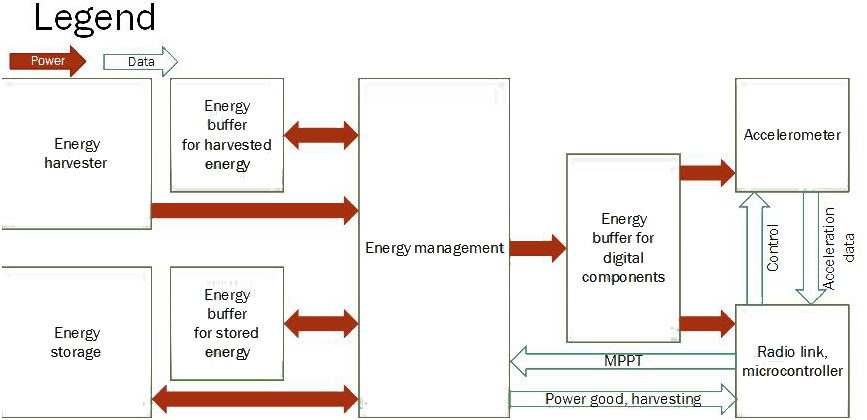
\includegraphics[height=6cm]{images/system_block_diagram.jpg}
\end{center}
\caption{\label{system_blog_diagram} Block diagram of complete system.}
\label{liitekuva}
\end{figure}


\subsection{Electrical design}
The analog sections of circuit were simulated using LTSpice IV {\color{red} reference}. Accelerometer and bluetooth module were modelled as parallel current sinks which took energy from the circuit in pulses. Energy harvesting was simulated as a high.impedance AC voltage source. 
Battery was modelled as a voltage source with high-value capacitor and low-value resistor in series.

\subsection{Energy harvester}
\subsubsection{Overview of available methods}
Several different methods for harvesting were experimented with to find optimal solution for the application. After initial review of energy harvesting methods, it was obvious that methods which use mechanical energy as their power source are best suited to application. Different approaches are piezoelectronic, electrostatic, electromagnetic and microelectromechanical systems (MEMS). 

Piezoelectronic systems use {\color{red} review of physical basis of piezos}. Their power output is rather limited, and it is uncertain if usable output of a few milliwatts could be reached with reasonable sized / priced element stack. However, the elements are stackable, so power output can be scaled as needed if higher cost of system is allowable.

Electrostatic devices charge plates of capacitor and use mechanical vibration to vary the structure of a capacitor. As the capacitance value changes with the structure, energy can be harvested from increased potential energy in capacitor. Drawback of this method is the required control electronics and high polarization voltages needed for maximal efficiency {\color{red} cite Electrostatic conversion for Vibration Energy harvesting}. There are also electrostatic methods which use *electrets*, Electronic Magnets. THese electrects hold constant charge and polarization for years and they can be used in electrostatic harvesters which do not require an external exitation source. While electrostatic harvesters have reached the required power levels, they are not readily available at the moment. Vibration characteristics of tyre pose additional challenges to electrostatic harvesters, as the plates must be protected against contact to one another during shocks. 

Electromagnetic harvesters utilise vibration to move a magnet inside a coil. The movement of a magnet causes a changing magnetic field, which gets coupled to coil. Coil opposes the change in magnetic field by inducing electrical current in device. A device could be built with a spring-loaded magnet to balance out the static acceleration of a tyre. An added bonus to spring loaded mechanism would be the utilisation of resonant frequency of the spring-mass system: as the system gets a shock, some of the energy would be in correct frequency rate to make the magnet oscillate inside coil allowing generation of energy until next shock. The coil will also function  as a dampener to system, so no extra dampening is required. Primary concern is the survivability of a magnet in an environment with heavy shocks and vibration. 

An in-depth overview is done to broadband piezoelectric and electromagnetic methods, as they are best fits to environment and previous work has proved it's possible to generate required amounts of power with both methods.

\subsubsection{Broadband piezoelectric harvesting}
A common approach to piezoelectric harvesting is to configure the element as a cantilever and tune the resonant frequency of the system to dominant frequency of the surrounding environment. This tuning is done by attaching a mass to the end of cantilever. This sort of tuned approach is not feasible in the environment of the tire, as the piezoelectric harvester has to be compliant enough to vibrate in low accelerations of few g's and stiff enough to withstand centripetal shocks of several hundred g's. {\color{red} Cite}. 

The harvester is instead configured as a patch fixed to surface of the tire from one end. Other end will be freely moving to allow flexing and compressing for the element as recommended by Thunder and Lightning piezos {\color{red} cite datasheet / app note}. Usually this kind of approach is avoided, as it is less efficient at harvesting energy from surroundings. Tyre however has plenty of energy especially at higher speeds, so the efficiency of the harvester doesn't have to be high.

\subsubsection{Resonant electromagnetical harvesting}
As the electromagnetical harvester does not bend in any direction, it's better suited to be built straight up along Z-axis. The structure can be made strong enough to survive the shocks present without compromising on the harvester operation. A magnet can be suspended with a spring inside a coil. When there is vibration in addition to relatively constant centripetal force, the magnet will move along the shaft of the coil and generate electricity. 

A non-linear spring can be utilised to keep the magnet as well centered as possible over a wide range of tyre speeds. This non-linearity could also be used to shift the resonant frequency of generator to track the frequency of vibration inside the tyre. 

 




